\documentclass[aspectratio=169]{beamer}
\usetheme{Skudai}

\usepackage[utf8]{inputenc}
\usepackage{helvet}
\usepackage{amsmath}
\usepackage{verbatim}

\title{\LaTeX{} \textit{Beamer Template} Universitas Mataram}
\subtitle{\textit{Subtitle}}
\author{Muhammad Erfan, S.Pd., M.Pd.}
\date{\today}
\institute{email: \url{muhammaderfan@unram.ac.id}}

\begin{document}
%\setbeamertemplate{headline}{}
%\setbeamertemplate{footline}{}
\begin{frame}[plain]
\titlepage
\end{frame}

\begin{frame}{Table of Contents}
    \tableofcontents
\end{frame}

\section{Introduction}
\begin{frame}
\frametitle{Frame Title}
\framesubtitle{Frame Subtitle}
Itemize
\begin{itemize}
    \item First Item
    \item Second Item
    \item Third Item
\end{itemize}
\end{frame}

\section{LaTex}
\subsection{Pengenalan LaTex}
\begin{frame}
\frametitle{\LaTeX}
\framesubtitle{Apa itu \LaTeX?}
\begin{itemize}
    \item \TeX\ adalah bahasa pemrograman yang diciptakan khusus dan menjadi bagian utama dari sistem pencetakan \textit{(typesetting system)} yang akan menghasilkan dokumen (teks, gambar, tabel, maupun notasi matematis) yang \textbf{berkualitas tinggi}.
    \item \TeX\ diciptakan oleh Prof. Donald Knuth sekitar tahun 1978.
    \item Pada tahun 1985, Leslie Lamport di Digital Equipment Corporation kemudian menciptakan \LaTeX, yaitu \textit{user interface} dari \TeX.
    \item Saat ini, \TeX\ maupun \LaTeX\ tersedia bebas di internet dan dapat digunakan oleh perseorangan maupun tim.
\end{itemize}
\end{frame}

\begin{frame}
\frametitle{\LaTeX}
\framesubtitle{Kenapa Menggunakan \LaTeX?}

\begin{exampleblock}{Keunggulan}
\begin{enumerate}
    \item Memiliki kemampuan yang baik dalam menyiapkan tulisan teks, formula matematis, tabel, gambar dll.
    \item Kemudahan penggunaan oleh penulis naskah, apa yang dikehendaki, itulah yang akan dihasilkan.
    \item Dapat digunakan dalam berbagai platform baik Windows, Linux, Mac OS, dll.
    \item Tersedia dalam bentuk online maupun software offline yang dapat digunakan perseorangan maupun tim.
    \item Tersedia secara luas dan bebas.
\end{enumerate}
\end{exampleblock}
\end{frame}

\begin{frame}
\frametitle{\LaTeX}
\framesubtitle{Kenapa Menggunakan \LaTeX?}

\begin{alertblock}{Kekurangan}
\begin{enumerate}
    \item Cukup sulit bagi pemula yang baru mengenal \LaTeX.
    \item \LaTeX\ membutuhkan ketelitian yang tinggi karena pembuatan dokumen ini sangat terstruktur.
\end{enumerate}
\end{alertblock}
\end{frame}

\subsection{Cara Kerja LaTex}
\begin{frame}[fragile]
\frametitle{\LaTeX}
\framesubtitle{Bagaimana \LaTeX\ bekerja?}
\begin{itemize}
    \item Pertama-tama kita susun dokumen dalam bentuk perintah-perintah yang mendeskripsikan struktur dan arti yang diinginkan.
    \item Kemudian program \LaTeX\ memproses dokumen dan perintah kita dalam bentuk dan format yang kita inginkan.
    \item Contoh:
    \verb|Selamat Datang di FKIP \textbf{Universitas Mataram}|
    \item Menjadi: \\
    Selamat Datang di FKIP \textbf{Universitas Mataram}
\end{itemize}
\end{frame}

\begin{frame}[fragile]
\frametitle{\LaTeX}
\framesubtitle{Contoh Lain}
\begin{table}[]
\begin{tabular}{r|l}
\verb|\begin{itemize}|\\
\verb|\item Matematika|\\
\verb|\item Fisika|\\
\verb|\item Kimia|\\
\verb|\item Pramuka|\\
\verb|\end{itemize}| &
  \begin{minipage}[t]{0.4\textwidth}
    \begin{itemize}
    \item Matematika
    \item Fisika
    \item Kimia
    \item Pramuka
    \end{itemize}
  \end{minipage}
\end{tabular}
\end{table}
\end{frame}

\begin{frame}
\frametitle{Jadi...}
Jika pada \textbf{Microsoft Word} kita mengedit langsung dari yang terlihat, pada \LaTeX\ kita mendeskripsikan apa yang kita kehendaki menjadi perintah-perintah dan ketika di-\textit{compile} maka \LaTeX\ akan menerjemahkannya dan membuatnya sesuai dengan perintah.
\end{frame}

\begin{frame}
\frametitle{Online \LaTeX}
\begin{itemize}
    \item Membuat dokumen \LaTeX menggunakan online \LaTeX\ \textit{editor} tidak perlu menginstall software apapun
    \item Terlebih lagi dapat dimungkinkan untuk bekerja secara tim untuk mengedit dokumen yang sama
\end{itemize}
Beberapa \textit{online} \LaTeX\ \textit{editor} yang dapat digunakan diantaranya:
\begin{itemize}
    \item Overleaf (\url{http://www.overleaf.com/})
    \item ShareLaTeX (\url{http://www.sharelatex.com/})
    \item VerbTeX (\url{http://www.verbtex.com/})
    \item dll.
\end{itemize}
\end{frame}

\section{Overleaf}
\begin{frame}
\centering
\textbf{\Huge Overleaf}\\
\Large \url{https://www.overleaf.com/}
\end{frame}

\begin{frame}
\frametitle{Apa itu Overleaf?}
\begin{itemize}
    \item Overleaf adalah website yang digunakan untuk menulis dokumen dengan \LaTeX.
    \item Pada website ini hasil \textit{compile} dokumen \LaTeX\ akan secara otomatis ditampilkan
    \item Untuk hasil yang maksimal, dapat digunakan web browser.
    \begin{itemize}
        \item Google Chrome\\
        (\url{https://www.google.com/chrome/})
        \item Mozilla FireFox\\
        (\url{https://www.mozilla.org/en-US/firefox/new/})
    \end{itemize}
\end{itemize}
\end{frame}

\begin{frame}
\frametitle{\textbf{Overleaf}}
\begin{figure}
    \centering
    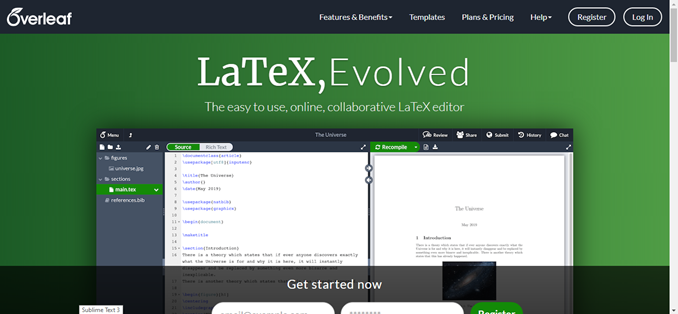
\includegraphics[width=0.9\textwidth]{gambar/overleaf.png}
\end{figure}
\end{frame}

\begin{frame}
\frametitle{\textbf{Overleaf}}
\framesubtitle{Keunggulan Overleaf}
\begin{figure}
    \centering
    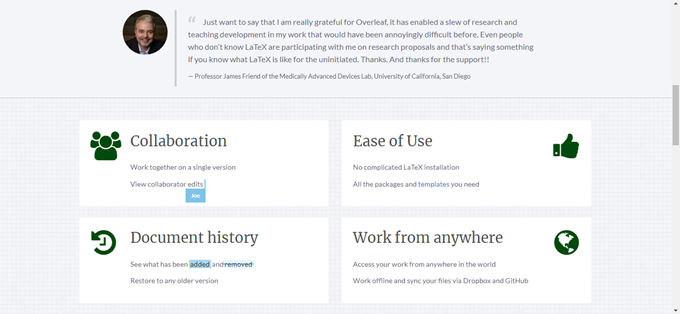
\includegraphics[width=\textwidth]{gambar/overleaf-2.png}
\end{figure}
\end{frame}

\begin{frame}
\frametitle{Template Artikel}
\framesubtitle{dengan \LaTeX\ di Overleaf}
Hal yang perlu diperhatikan!
\begin{itemize}
    \item Di Overleaf, sudah disediakan beberapa contoh template artikel di Jurnal Internasional (IOP, Springer, Elsevier, dll), kita tinggal mengeditnya.
    \item Untuk pengolahan tabel bisa menggunakan \textbf{Table Generator} (\url{https://www.tablesgenerator.com/})
    \item Untuk pengolahan rumus matematika bisa menggunakan \textit{codecogs.com} (\url{https://www.codecogs.com/latex/eqneditor.php})
    \item Untuk pengolahan Gambar bisa gunakan Paint atau pengolah gambar lain dengan output gambar dengan ekstensi .jpg, .png, .eps.
    \item Manajemen referensi bisa menggunakan \textbf{Mendeley} dengan \textit{export as bibtex} (.bib)
\end{itemize}
\end{frame}

\begin{frame}
\frametitle{\textit{Tables Generator}}
\framesubtitle{(\url{https://www.tablesgenerator.com/})}
\begin{figure}
    \centering
    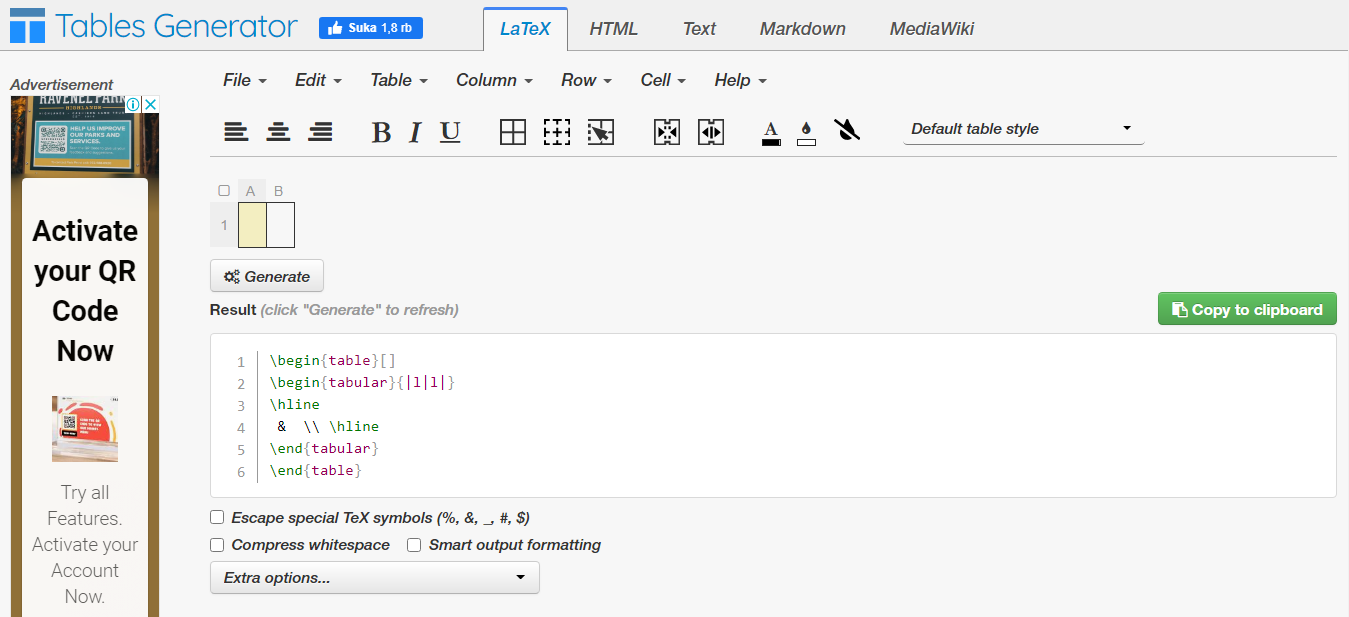
\includegraphics[width=\textwidth]{gambar/tablegen.png}
\end{figure}
\end{frame}

\begin{frame}
\frametitle{\LaTeX\ \textit{Equation Editor}}
\framesubtitle{(\url{https://www.codecogs.com/latex/eqneditor.php})}
\begin{figure}
    \centering
    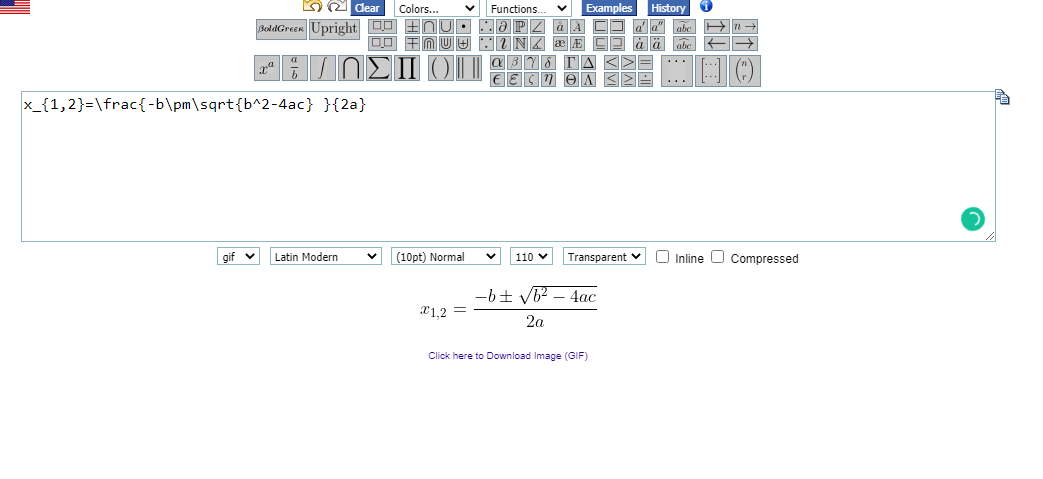
\includegraphics[width=\textwidth]{gambar/codecogs.png}
\end{figure}
\end{frame}

\begin{frame}[fragile]
\frametitle{\textit{Command-command} Penting!}
\framesubtitle{Berkaitan dengan Template Artikel pada \LaTeX}
\begin{itemize}
    \item Judul Artikel: \verb|\title{Judul Artikel}|
    \item Nama Pengarang: \verb|\author{Nama Pengarang}|
    \item Abstrak: \\
    \verb|\begin{abstract}|\\
        \verb|[..paste abstrak disini..]|\\
    \verb|\end{abstract}|
    \item Sitasi Menggunakan: \verb|\cite{namapengarang}|
    \item Bagian Artikel: \verb|\section{Introduction}|
    \item dll.
\end{itemize}
\end{frame}

\begin{frame}[fragile]
\frametitle{\textit{Error} pada \LaTeX}
\begin{itemize}
    \item \LaTeX\ dapat mengalami \textit{error} pada saat meng-\textit{compile} dokumen. Jika demikian, maka mungkin ada \textit{syntax} perlu perbaiki terlebih dahulu atau dokumen tidak dapat ditampilkan.
    \item Contohnya, jika terjadi kesalahan ketik \verb|\emph{}| dengan \verb|\meph{}|, maka \LaTeX\ akan terhenti dengan keterangan error yaitu: ''undefined control sequence''. Hal ini dikarenakan ''meph" bukan perintah yang dikenal.
\end{itemize}
\textbf{CATATAN:}
\begin{itemize}
    \item Jangan panik jika terjadi \textit{error}
    \item Sering-sering meng-\textit{compile} dokumen sehingga jika terjadi \textit{error} maka bisa segera ditangani.
\end{itemize}
\end{frame}

\begin{frame}
\frametitle{\LaTeX\ Template \textit{Tutorial}}
\framesubtitle{(\url{https://youtube.com/channel/UCnt9OCAfEzk4t0rbDOVH_QQ})\\(\url{https://bit.ly/latex-erfan})}
\begin{figure}
    \centering
    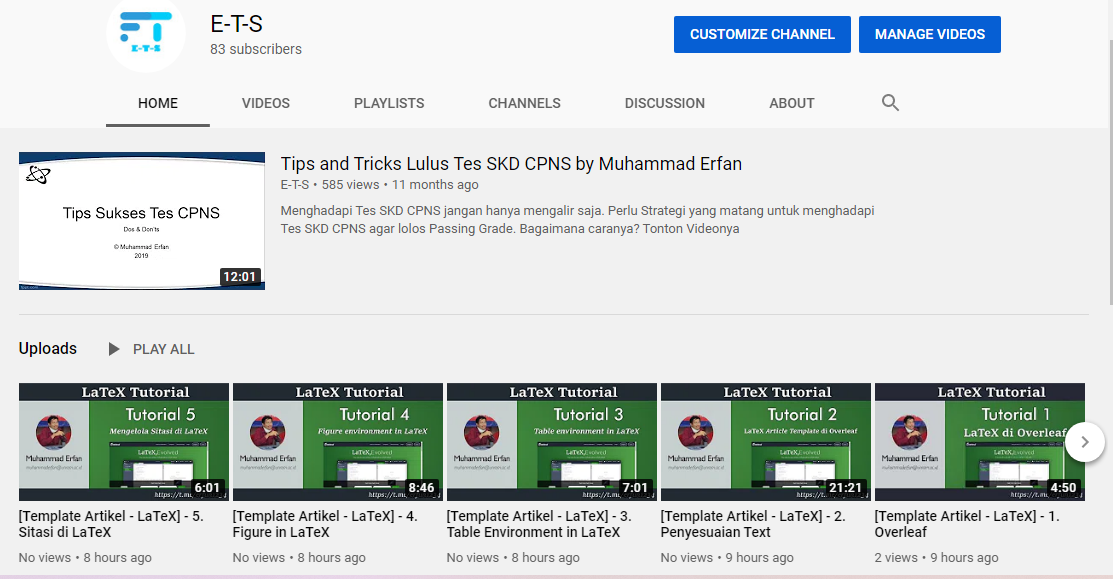
\includegraphics[width=\textwidth]{gambar/Youtube.png}
\end{figure}
\end{frame}

\begin{frame}
\centering
\textbf{\Huge Terima Kasih}\\ \textit{Ada pertanyaan?}
\end{frame}

\end{document}